\documentclass[UTF8,a4paper,zihao=-4]{ctexart}
\usepackage[a4paper,margin=2.0cm]{geometry}
\usepackage{amsmath,amssymb,booktabs,tabularx,array,multirow,graphicx,xcolor,enumitem,microtype}
\usepackage{hyperref,cleveref,fancyhdr,lastpage}
\usepackage[backend=biber,style=gb7714-2015]{biblatex}
\addbibresource{refs.bib}
\definecolor{EcoNavy}{HTML}{17324D}\definecolor{EcoTeal}{HTML}{168AAD}\definecolor{EcoOrange}{HTML}{E76F51}\definecolor{EcoGold}{HTML}{E9C46A}\definecolor{EcoGray}{HTML}{64748B}
\hypersetup{colorlinks=true,linkcolor=EcoTeal,citecolor=EcoTeal,urlcolor=EcoTeal,pdftitle={EcoSentinel答辩演讲稿}}
\pagestyle{fancy}\fancyhf{}\setlength{\headheight}{14.5pt}\lhead{EcoSentinel 环境监测与 AI 节能调控系统}\rhead{答辩演讲稿}\cfoot{\thepage/\pageref{LastPage}}
\newcommand{\placeholder}[1]{\textcolor{EcoOrange}{\textbf{【待补：#1】}}}
\newcommand{\metric}[2]{\textcolor{EcoTeal}{\textbf{#1}}\,（#2）}
\title{\vspace{-1cm}\textcolor{EcoNavy}{EcoSentinel 环境监测与 AI 节能调控系统}\\[0.4em]\Large 科研风格答辩演讲稿与逐页讲解提纲}
\author{参赛团队：\placeholder{团队名称、成员与指导教师}}\date{\placeholder{比赛名称与答辩日期}}
\begin{document}
\maketitle
\begin{center}\small 建议演讲时长：\placeholder{8--12 分钟}\quad |\quad 版本：v1.0（可编辑稿）\end{center}
\begin{abstract}
本稿面向 EcoSentinel 环境监测与 AI 节能调控系统的竞赛答辩，围绕“问题—方法—系统—验证—边界—贡献”组织口头表达。项目以 ESP32-S3 感知执行节点、Python 边缘运行时、FastAPI 数据服务和 React/Streamlit 可视化为主体，形成从环境感知、规则控制、AI 建议到审计反馈的闭环。当前数字孪生基线实验在固定参数、固定随机种子下得到基线模式 81.48 kWh、节能模式 57.18 kWh，节电率 29.8\%，舒适度 82.1\%。这些数字属于仿真结果，不替代真实平台实测；现场答辩时应将\placeholder{实测电表、温湿度、通信时延和故障恢复数据}补入。
\end{abstract}
\section{开场：从“我敢闯，我会创”到真实建筑问题}
各位评委老师好，我们展示的项目是 EcoSentinel 环境监测与 AI 节能调控系统，项目中文名称为“穹顶之光”。2026 中国国际大学生创新大赛的主题是“我敢闯，我会创”，高教主赛道设置了“人工智能+”等项目类型，并强调真实问题、创新实践、产教融合和成果转化。我们的切入点不是把 AI 当作宣传标签，而是把它放进一个可以演示、可以审计、也可以逐步落地的建筑节能闭环中。

它关注一个看似日常、但很容易被低估的问题：在保证环境舒适和设备安全的前提下，能否让一个小型建筑空间的监测、控制和能耗管理变得更连续、更可解释、更容易复现？本稿中的竞赛资格、团队人数、知识产权和成员贡献信息，仍需根据正式通知和校级审核材料补齐。

传统方案往往把传感器、继电器、云端看板和控制逻辑拼接在一起，系统可以“运行”，却不一定能够回答三个工程问题：第一，数据异常时系统是否会安全降级；第二，AI 给出建议时谁拥有最终执行权；第三，节能结果是一次偶然的演示，还是能够由固定参数和版本重新得到的实验结果。

建筑领域节能与数字化运行管理已经成为重要方向。国际能源署将建筑数字化优化视为提高运行效率的重要路径\cite{iea_efficiency_2025}；我国 2024 年发布的建筑领域节能降碳工作方案也强调建筑运行节能管理、能耗统计核算和数字化智能化平台建设\cite{china_building_efficiency_2024}。因此，本项目不是单纯做一个“温湿度显示器”，而是尝试把感知、控制、能耗核算和软件工程质量放在同一个可验证框架中。
\section{第二部分：项目的核心思路}
我们的核心思路可以概括为一句话：\textbf{让 AI 负责提出建议，让规则、安全策略和审计链路负责决定系统能否执行。}

系统首先由 ESP32-S3 节点采集温度、湿度、光照、空气质量和电能等信息，并承担继电器、蜂鸣器、窗帘或其他执行器控制。边缘层不依赖网络才能完成基本控制，因此在网络不稳定或 AI 不可用时，仍由本地规则保证安全运行。AI 顾问只输出结构化候选命令，命令还需要经过语法解析、设备白名单、参数范围、权限模式、限频和审计检查。

这一设计借鉴了物联网系统中轻量消息传输和边缘自治的思想。MQTT 5.0 是面向受限环境的发布/订阅消息传输协议，强调低开销和通信解耦\cite{mqtt5}；ESP32-S3 提供双核 LX7、2.4 GHz Wi-Fi、Bluetooth LE 以及多种传感器和控制接口，适合作为本项目的节点级平台\cite{esp32s3}。
\begin{figure}[htbp]\centering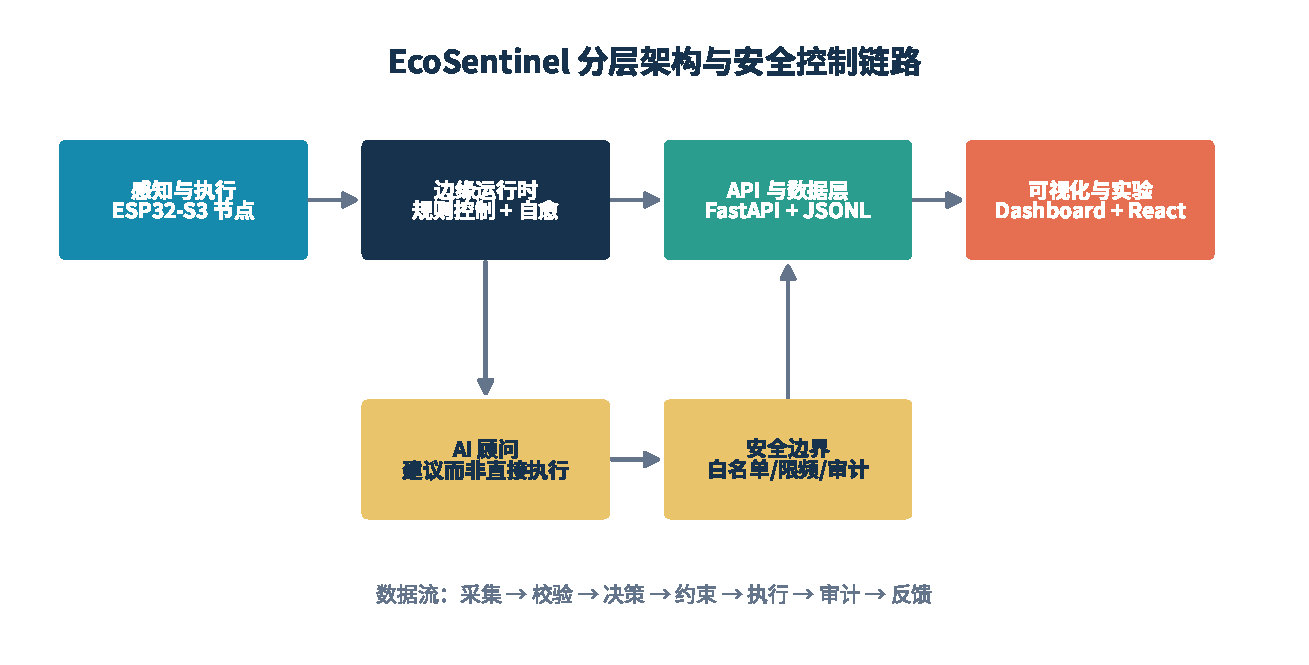
\includegraphics[width=0.97\linewidth]{figures/architecture.pdf}\caption{EcoSentinel 分层架构与安全控制链路。}\label{fig:architecture}\end{figure}
\section{第三部分：系统如何工作}
系统运行过程可以分为六步。第一步是感知：节点按照固定周期读取传感器，并形成带时间戳的遥测记录。第二步是校验：边缘层检查字段类型、时间顺序、缺失值和异常范围。第三步是决策：本地控制器根据温度滞回、设备最小运行时间和最小停止时间等规则生成计划。第四步是建议融合：AI 可以给出受限候选动作，但不能绕过规则保留边界。第五步是执行与审计：动作经编译后发送给执行器，同时记录事件、来源、结果和失败原因。第六步是反馈：数据进入 JSONL 实验记录、API 服务和可视化界面。

在软件结构上，本项目已经完成 P0--P11 的渐进式重构。重构遵循“先冻结行为、再建立边界；先补测试、再移动代码；保留旧入口、分阶段可回滚”的原则。API 层采用仓储、服务和 schema 分层；应用层拆分运行时、控制周期、决策与富化；AI 层拆分模型、解析器、回退策略和熔断器；固件由单文件 sketch 拆分为 header-only 模块，同时保持串口协议字段名不变。
\section{第四部分：实验设计与结果}
为了避免把仿真结果误说成实测，我们把验证分为三层。第一层是软件回归，检查接口、类型、异常数据和兼容入口。第二层是数字孪生基线实验，在固定时间步长、持续时间和随机种子下比较 baseline 与 saving 两种模式。第三层是真实硬件验证，需要在 Arduino IDE 或 PlatformIO 中编译固件，并在实际传感器、继电器、Wi-Fi/MQTT 环境中回放协议和测试故障恢复。

当前数字孪生实验采用 3 天时长、300 秒步长和随机种子 42。仿真结果如下。\textbf{请注意：这些结果应在答辩最终版中注明“数字孪生仿真”，并用实测结果补充现场性能结论。}
\begin{table}[htbp]\centering\caption{固定参数数字孪生基线结果}\label{tab:simulation}\begin{tabular}{lrr}\toprule 指标 & 基线模式 & 节能模式\\\midrule 累计能耗 / kWh & 81.48 & 57.18\\ 节省电量 / kWh & \textemdash & 24.30\\ 节电率 / \% & \textemdash & 29.8\\ 平均舒适度 / \% & 82.1 & 82.1\\\bottomrule\end{tabular}\end{table}
\begin{figure}[htbp]\centering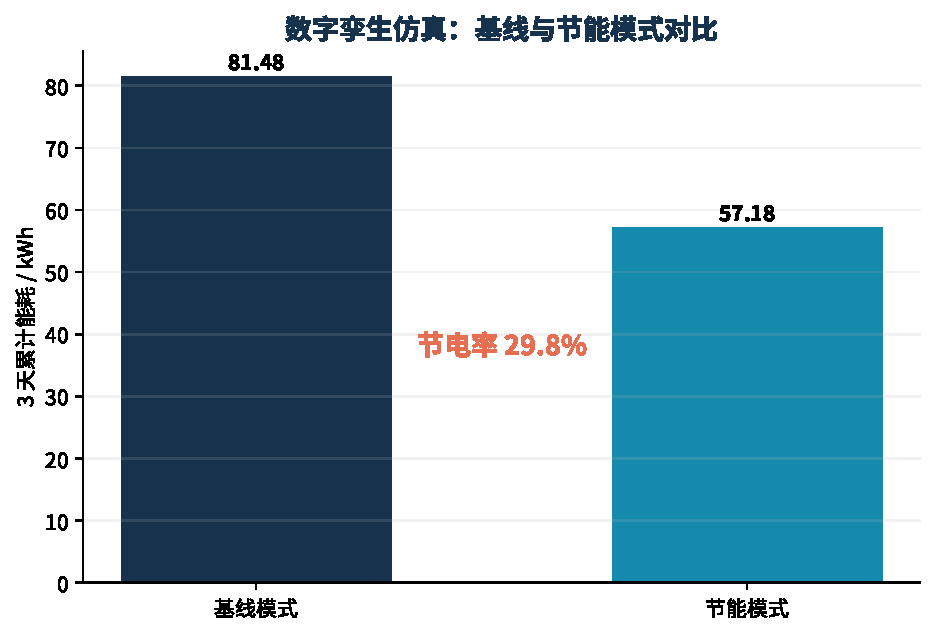
\includegraphics[width=0.72\linewidth]{figures/energy_comparison.pdf}\caption{基线与节能模式的累计能耗比较。}\label{fig:energy}\end{figure}

能耗指标按照功率随时间积分计算：
\begin{equation}\label{eq:energy} E_{\mathrm{kWh}}=\frac{1}{3.6\times10^{6}}\sum_{i=1}^{n}P_i\Delta t_i, \qquad R_{\mathrm{save}}=\frac{E_{\mathrm{base}}-E_{\mathrm{save}}}{E_{\mathrm{base}}}\times100\% .\end{equation}
其中，\(P_i\) 为第 \(i\) 个时间片的功率，\(\Delta t_i\) 为时间片长度。真实实验中还应记录电表型号、采样周期、校准方式、环境初始状态和数据缺失比例。\placeholder{补充实测实验表编号、平台照片编号和统计置信区间}。
\section{第五部分：项目与竞赛方向的匹配}
\begin{figure}[htbp]\centering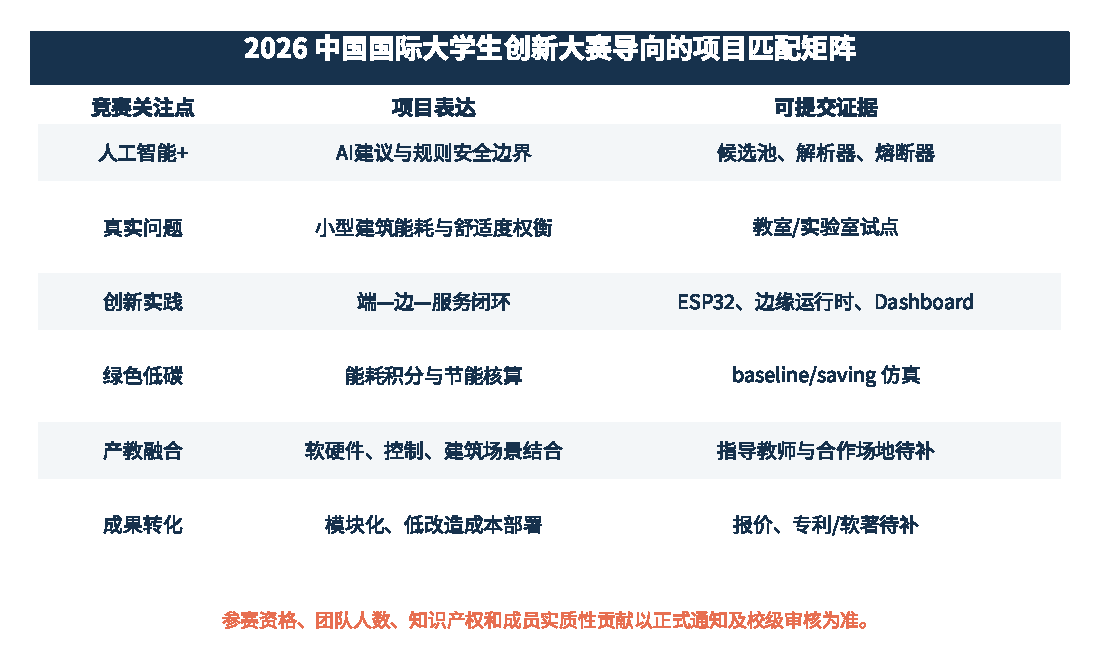
\includegraphics[width=0.93\linewidth]{figures/competition_match.pdf}\caption{项目特征与 2026 中国国际大学生创新大赛关注点的匹配矩阵。}\label{fig:competition}\end{figure}
从竞赛表达看，项目应同时回答“为谁解决什么问题”“为什么必须采用人工智能”“如何证明不是概念演示”“能否形成可转化产品”四个问题。我们的答案是：面向教室、实验室、办公室等小型空间，利用传感器和边缘计算持续感知环境，以 AI 生成候选建议、以规则和安全编译器决定是否执行，并用能耗记录和异常审计形成证据链。\textbf{人工智能在这里是受约束的决策辅助，不是绕过工程边界的自动驾驶。}

\begin{table}[htbp]\centering\small\caption{竞赛答辩中的“主张—证据—边界”表达方式}\begin{tabularx}{\linewidth}{>{\bfseries}p{0.22\linewidth}X p{0.25\linewidth}}\toprule 主张 & 当前证据 & 不能过度表述的边界\\\midrule
系统能稳定运行 & 148 项 Python 回归测试、compileall、前端质量门禁与 CI & 真实 ESP32 长时间运行仍待完成\\
系统能够节能 & 固定参数数字孪生：81.48 与 57.18 kWh，节电率 29.8\% & 仿真不等于真实建筑节能率\\
AI 使用安全 & 候选命令、白名单、范围、限频、熔断和回退链路 & 仍需台架故障注入记录与现场审计样本\\
项目具有转化潜力 & 模块化硬件、边缘优先、低改造思路与多场景路线 & 报价、专利/软著、合作场地和客户访谈待补\\\bottomrule\end{tabularx}\end{table}

\section{第六部分：场景、对比与产品化表达}
传统定时控制实现简单，却看不见真实占用和环境变化；纯云端 AI 具有灵活性，却依赖网络并面临物理执行边界；纯本地规则可靠，但难以吸收复杂建议。EcoSentinel 的差异不在于宣称某个单一算法“全面领先”，而在于把连续感知、边缘自治、受约束 AI 和可追溯实验放在同一产品结构中。
\begin{figure}[htbp]\centering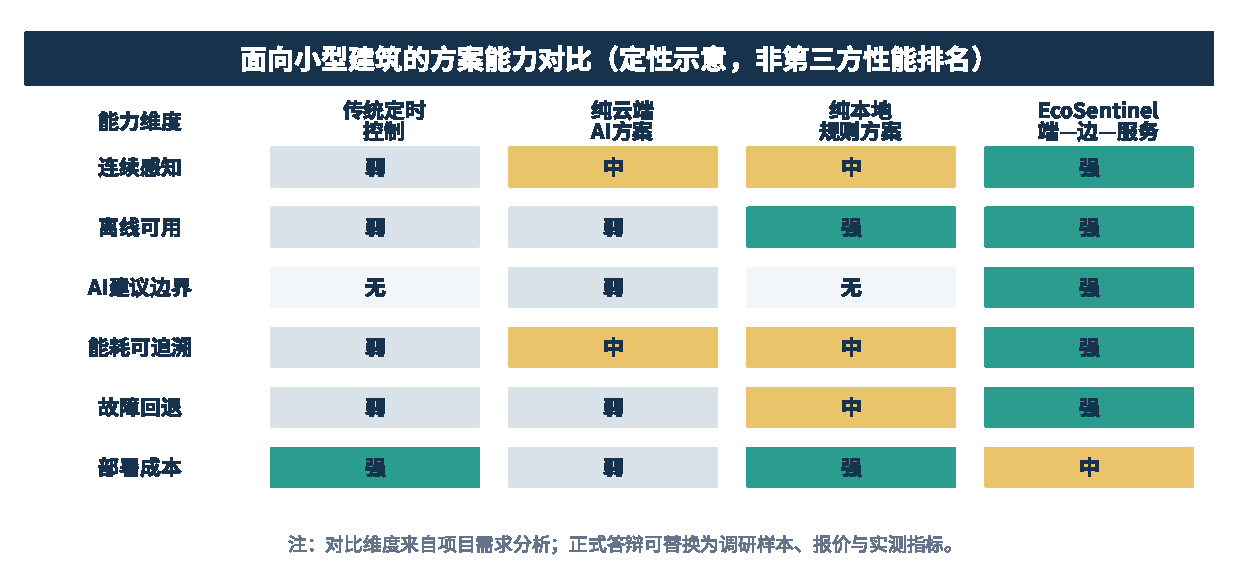
\includegraphics[width=0.96\linewidth]{figures/solution_comparison.pdf}\caption{传统定时、纯云端 AI、纯本地规则与 EcoSentinel 的定性能力对比。}\label{fig:comparison}\end{figure}
\begin{figure}[htbp]\centering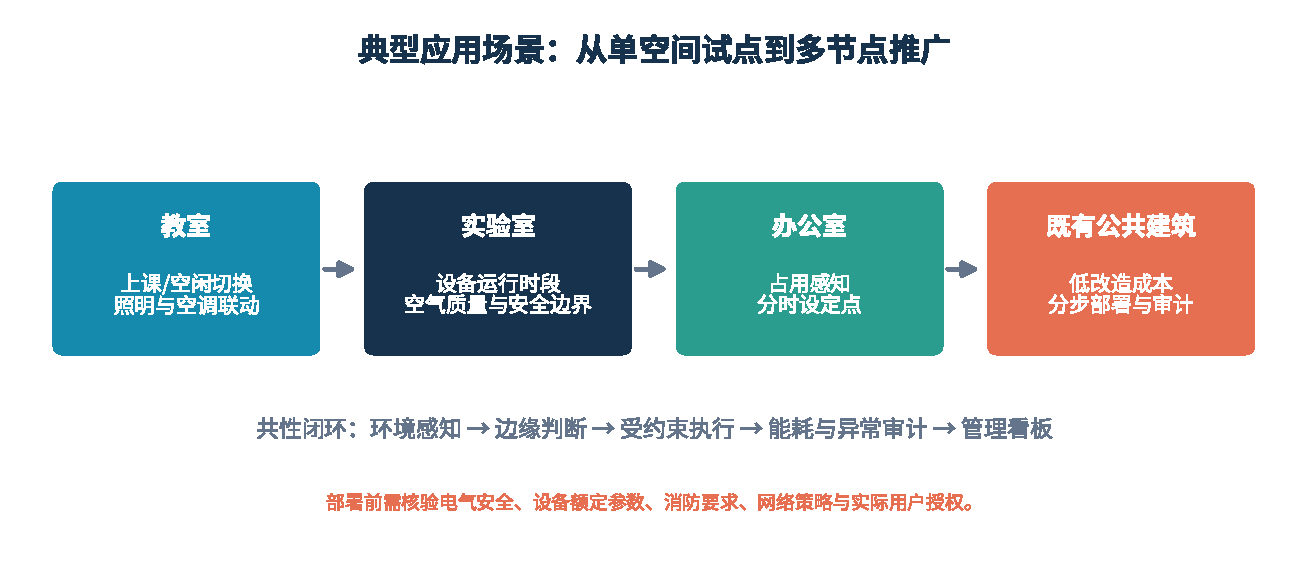
\includegraphics[width=0.96\linewidth]{figures/application_scenarios.pdf}\caption{从教室、实验室和办公室到既有公共建筑的典型应用场景。}\label{fig:scenes}\end{figure}
答辩演示建议按“看见问题—接入节点—展示异常—触发规则回退—查看能耗记录”的顺序进行。现场若尚未完成真实硬件闭环，应明确演示的是软件仿真或协议回放，不将模板曲线和空白实测点包装成现场成果。

\section{第七部分：从节能数字到产品化路径}
数字孪生实验用于验证控制策略和复现流程；项目原始材料中曾出现 15\%--25\% 综合节能率、日耗电量和年度收益等测算口径，但在补齐原始电表记录、设备额定功率、运行时长、电价、地区排放因子和统计方法前，只能作为\textbf{待核验测算}，不能与本稿的 29.8\% 仿真结果混列。
\begin{figure}[htbp]\centering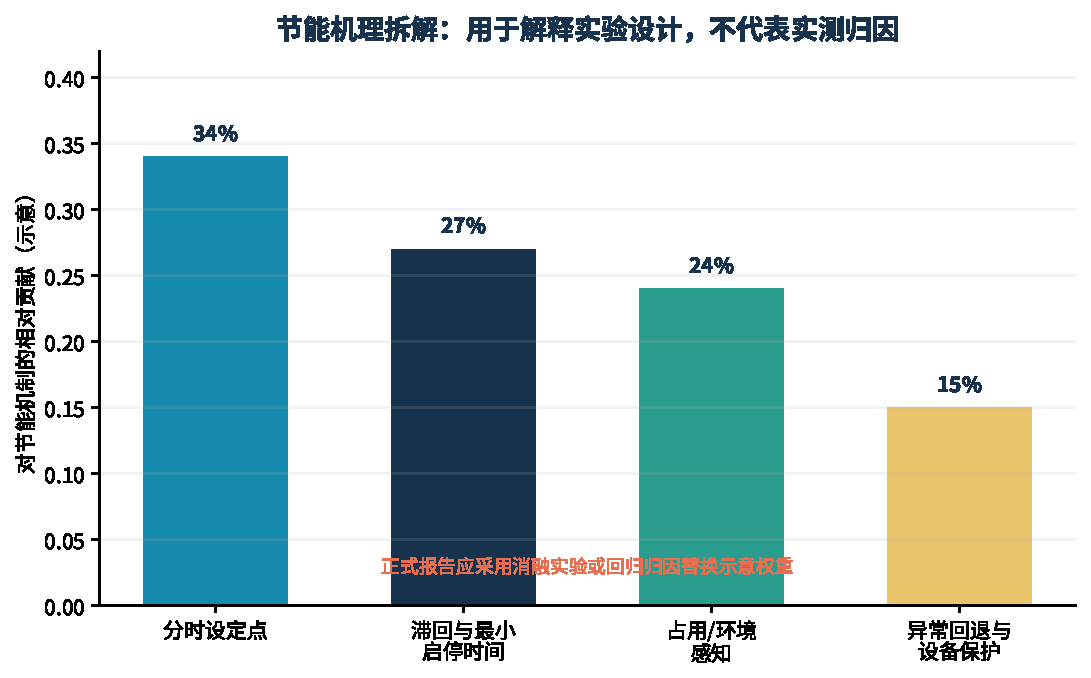
\includegraphics[width=0.78\linewidth]{figures/energy_contribution.pdf}\caption{节能机理拆解示意；权重不代表实测归因。}\label{fig:contribution}\end{figure}
\begin{figure}[htbp]\centering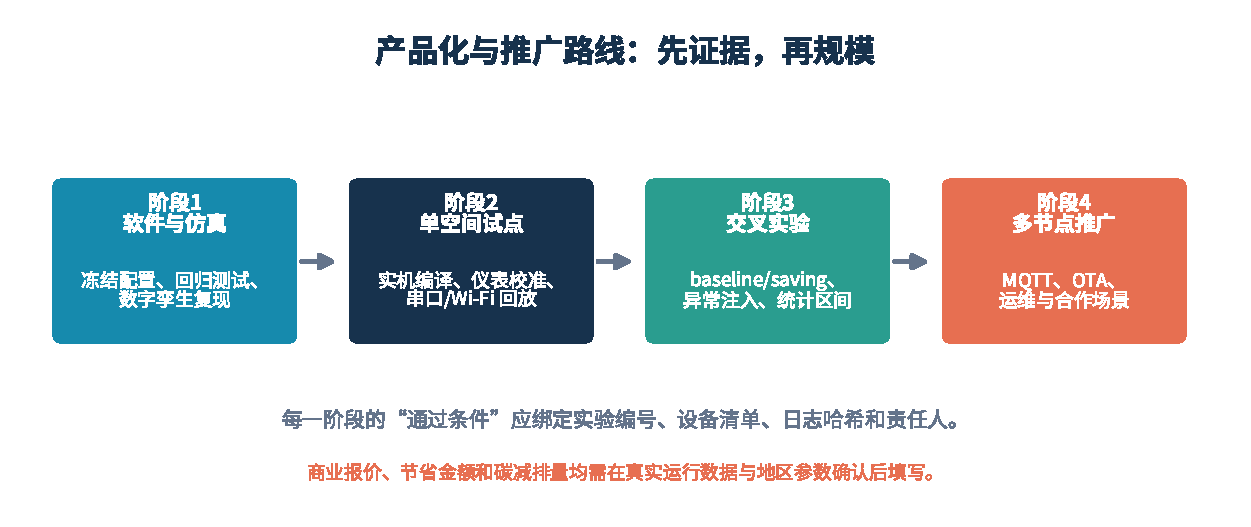
\includegraphics[width=0.96\linewidth]{figures/deployment_roadmap.pdf}\caption{产品化与推广路线：先完成证据，再扩展节点规模。}\label{fig:roadmap}\end{figure}
\begin{table}[htbp]\centering\small\caption{建议补齐的产品化与团队信息}\begin{tabularx}{\linewidth}{>{\bfseries}p{0.25\linewidth}X}\toprule 项目 & 待补与建议证据\\\midrule
用户与场地 & \placeholder{访谈对象、场地面积、设备清单、试点授权}\\
团队分工 & \placeholder{硬件、嵌入式、算法、前端、运营与答辩分工}\\
知识产权 & \placeholder{专利/软著名称、申请号、成员实质性贡献}\\
成本收益 & \placeholder{BOM、安装工时、运维成本、电价与回收期假设}\\
合作转化 & \placeholder{指导教师、企业/场地合作、试点协议、反馈记录}\\
\bottomrule\end{tabularx}\end{table}

\section{第八部分：安全与可靠性}
本项目把安全边界放在 AI 之前。设备离线时进入保护策略；规则控制保留关键继电器；AI 命令必须满足 schema、白名单、范围和速率限制；连续超时或解析失败时触发回退策略和熔断；所有动作进入审计日志。这样的结构不是为了让系统“看起来更智能”，而是为了避免一个不可解释的建议直接变成不可逆的物理动作。

在工程质量方面，远程主分支已通过 Python 测试、编译检查、确定性仿真、React lint/typecheck/build 以及 gitleaks 扫描。GitHub Actions 将这些检查固化为提交门禁。该做法与持续集成的基本思想一致：每次提交都自动构建和测试，从而尽早发现回归问题\cite{github_actions}；gitleaks 则用于发现仓库中可能存在的硬编码密钥、令牌和密码\cite{gitleaks}。
\begin{figure}[htbp]\centering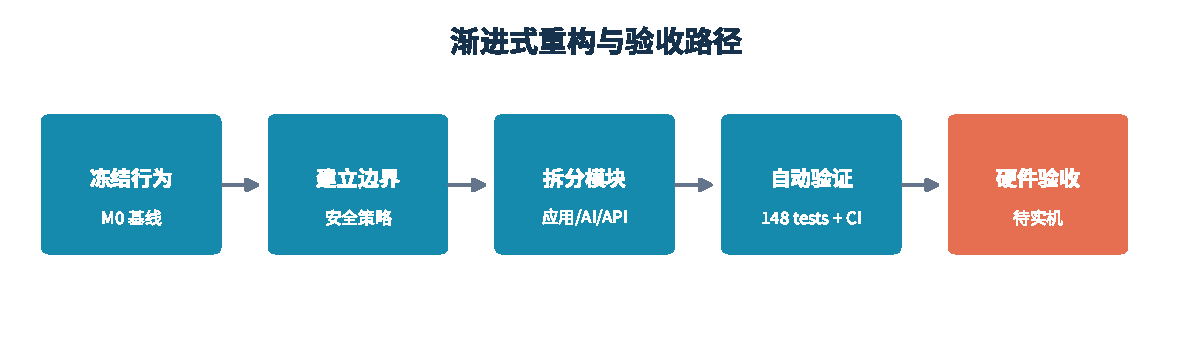
\includegraphics[width=0.97\linewidth]{figures/validation_pipeline.pdf}\caption{从行为冻结到软件门禁和硬件验收的验证路径。}\label{fig:pipeline}\end{figure}
\begin{figure}[htbp]\centering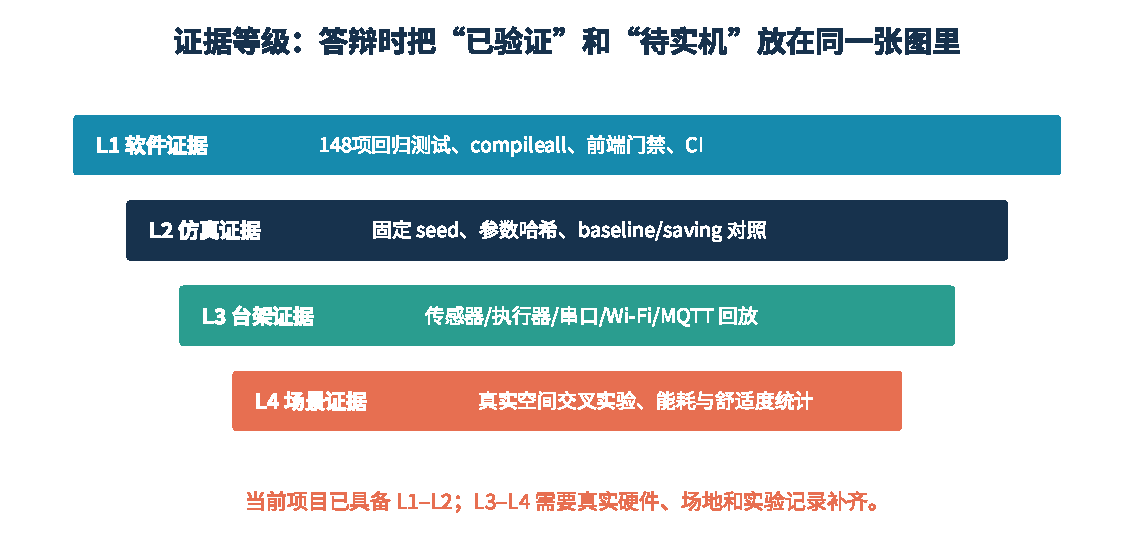
\includegraphics[width=0.92\linewidth]{figures/evidence_hierarchy.pdf}\caption{项目证据等级：软件、仿真、台架和场景四层证据分开报告。}\label{fig:evidence}\end{figure}

本项目的贡献主要有三点。第一，形成了面向小型建筑环境的端—边—云协同原型，把感知、控制、能耗和可视化放进同一条数据链路。第二，建立了 AI 建议与物理执行之间的安全隔离，强调规则优先、可回退、可审计。第三，把代码重构和实验可复现性作为项目成果的一部分，而不是演示结束后的附属工作。

我们也诚实说明项目边界。当前节能率和舒适度数字来自数字孪生仿真，不能直接等同于真实建筑的长期节能收益。真实硬件上的传感器漂移、执行器延迟、无线丢包、设备额定功率和用户行为都会影响结果。后续工作包括完成 ESP32 实机编译和协议回放，采集连续运行数据，开展 baseline/saving 交叉实验，并用\placeholder{置信区间、效应量和显著性检验}报告结论。
\section{结束语}
EcoSentinel 的目标不是把所有控制权交给 AI，而是让智能建议在清晰的工程边界内产生价值。我们希望通过可复现的实验、可追踪的软件结构和可回退的控制链路，让节能系统不仅能够运行，而且能够被解释、被验证、被维护。

我的汇报到这里，谢谢各位老师，欢迎批评指正。
\section*{答辩现场可替换数据清单}
\begin{tabularx}{\linewidth}{>{\raggedright\arraybackslash}p{0.28\linewidth}X}\toprule 项目 & 待补内容\\\midrule 团队信息 & \placeholder{学校、团队、成员、指导教师、赛道}\\ 实物信息 & \placeholder{传感器型号、继电器型号、功率计型号、固件版本}\\ 实测指标 & \placeholder{运行时长、能耗、节电率、舒适度、时延、丢包率}\\ 图片材料 & \placeholder{实物照片、接线图、现场运行截图、平台界面截图}\\ 竞赛信息 & \placeholder{奖项、专利/软著、指导意见、答辩时限}\\\bottomrule\end{tabularx}
\printbibliography
\end{document}
